\section{Method}

\paragraph{Data and task.}

We use 12 document contexts from six diplomatic event groups, including CMFA PressCon \citep{mochtak2021corpus} and Security Council discourse. Training covers the Korean Peninsula, South Sudan, and Kashmir (six contexts); development uses Gaza (two); testing uses Syria and Iran (four). Passages about ceasefires, reciprocal measures, and commitments guide synthetic bilateral negotiations. One party offers to maintain its measure for $x\in\{1,2,3\}$ weeks if the counterpart maintains its measure for $y\in\{1,2\}$ weeks. Durations, payoffs, types, and responses are researcher-defined.

For example, a peninsula briefing links suspending nuclear and missile activities to suspending military exercises. These reciprocal measures become the parties' actions. Documents supply the issues and commitment language; synthetic durations and costs determine acceptance.

\paragraph{State, actions, and reward.}

The agent has at most five decisions and cannot observe the counterpart's type, $\tau\in\{S,H\}$. It observes the offer, acceptance, commitments, costs, and belief $b_t=P(\tau=H)$. Eleven actions cover ambiguity, signaling, a private question, six conditional offers, ratification, and withdrawal. Questions provide noisy type cues; offer responses also reveal information. Ratification requires observed acceptance and own utility at least as high as the outside option.

Specifically, an agreement gives $u_A=0.5y-0.18x$, and the counterpart accepts when $u_B=0.35x-c_\tau y+\delta z\geq0$, where $z$ records a signal and $c_\tau$ determines the cost of reciprocal measures. A signal therefore changes an incentive; a question changes information. For response likelihoods $L_H$ and $L_S$, the public belief becomes
\begin{equation}
 b_{t+1}=\frac{b_tL_H}{b_tL_H+(1-b_t)L_S}.
\end{equation}
Equal response likelihoods leave the belief unchanged. Step rewards are
\begin{equation}
 r_t=d_tu_{\mathrm{end}}-0.01-c^{\mathrm{act}}_t-0.005e_{t+1}^2,
\end{equation}
where $d_t$ marks termination, $e$ counts rejected offers, and $c^{\mathrm{act}}_t$ sums question, signal, rejection, reversal, and invalid-action charges. Terminal utility is $u_A$ at agreement or 0.12 at withdrawal or expiration, paid once. We report $\sum_t r_t$. Appendix~\ref{app:environment} gives all costs and transition rules.

\paragraph{Shared language execution.}

GPT-5.6 Luna generates three styles per context--action pair, yielding 396 utterances. A separate Luna call interprets their function, reciprocal terms, and stated cost. These meanings determine transitions; interpretation mismatches are retained. All controllers share these utterances and templated counterpart replies, separating action selection from language realization.

\paragraph{Strategic controllers.}

We compare Random, a development-selected signal-first Heuristic, an immediate-reward Bandit, and PPO \citep{schulman2017ppo}. An exact belief-state planner maximizes expected net utility under the declared rules without seeing the true type. We distill its action values from training contexts and configurations, then refine the policy with PPO. Direct Luna (reasoning \texttt{none}) and Sol (\texttt{none}/\texttt{medium}) receive the public state and numerical rules.

The planner solves response branches by backward recursion. Following policy distillation and expert-guided learning \citep{rusu2016distillation,anthony2017expert}, we train on 43,440 public states from planner and exploratory trajectories. After 2,400 supervised updates, PPO refines the network. Deployment selects the highest-scoring action from 31 public features.

Planner values $Q_T(s,a)$ define the teacher distribution $p_T(a\mid s)\propto\exp(Q_T(s,a)/0.03)$. The supervised loss is
\begin{equation}
\begin{aligned}
\mathcal{L}={}&-\sum_a p_T(a\mid s)\log\pi_\theta(a\mid s)\\
&+\tfrac12\bigl(V_\theta(s)-\max_a Q_T(s,a)\bigr)^2.
\end{aligned}
\end{equation}
Policy targets preserve action preferences; value targets estimate return. PPO updates both using interaction rewards.

\section{Experimental Setup}

Initial evaluation crosses four contexts, 64 configurations, and three styles. Matched evaluation uses the first 16 configurations and one style (64 conditions); follow-up uses 64 new configurations and three styles. We take expectations over types and question responses, then average within and across event groups. Bandit and base PPO receive 102,400 steps per seed; distillation adds teacher supervision. Learned results average three seeds, using final checkpoints and development-selected methods. Appendices~\ref{app:training} and~\ref{app:diagnostics} give settings and diagnostics.

Every matched controller encounters the same context, numerical rules, utterances, and response-branch probabilities. We enumerate nonzero branches rather than relying on a single sampled counterpart, so differences reflect action choices under the shared environment.

\section{Results}

\begin{table}[t]
\centering\small
\setlength{\tabcolsep}{3pt}
\begin{tabular}{lrrr}
\toprule
Controller & Utility & Agree. & Calls \\
\midrule
\multicolumn{4}{l}{\textit{A. Initial: 256 conditions, three styles}} \\
Random & -0.146 $\pm$ 0.001 & 11.0 & 0 \\
Bandit & 0.118 $\pm$ 0.001 & 23.8 & 0 \\
Heuristic & 0.419 & 94.8 & 0 \\
PPO & 0.358 $\pm$ 0.018 & 73.0 & 0 \\
Planner & 0.488 & 93.3 & 0 \\
\midrule
\multicolumn{4}{l}{\textit{B. Matched: 64 conditions, one style}} \\
Luna none & -0.368 & 24.3 & 3.949 \\
Sol none & -0.367 & 26.3 & 4.773 \\
Sol medium & 0.514 & 100.0 & 3.429 \\
Heuristic & 0.470 & 100.0 & 0 \\
PPO & 0.378 $\pm$ 0.012 & 81.9 & 0 \\
Distilled PPO & 0.475 $\pm$ 0.016 & 98.3 & 0 \\
Planner & 0.533 & 100.0 & 0 \\
\bottomrule
\end{tabular}
\caption{Policy comparison with fixed Luna utterances. Agreement is a percentage; calls are per negotiation for strategy selection. $\pm$: three-seed SD (evaluation seeds for Random). Panels use different conditions.}
\label{tab:policies}
\end{table}

\begin{figure}[t]
\centering
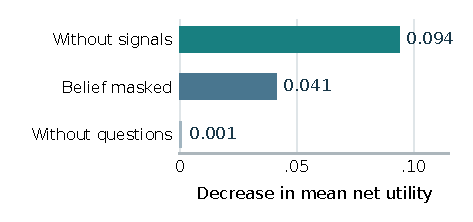
\includegraphics[width=\columnwidth]{figures/intervention_losses.pdf}
\caption{Evaluation-time interventions on distilled PPO. Losses are differences in three-seed mean utility on the follow-up conditions. Full values and seed variation appear in Table~\ref{tab:interventions}.}
\label{fig:interventions}
\end{figure}

Initially, PPO outperforms Random and Bandit but falls below the heuristic (Table~\ref{tab:policies}). In the matched comparison, the planner reaches 0.533 utility versus 0.514 for Sol medium. Distilled PPO reaches 0.475 versus 0.378 for base PPO and 0.470 for the heuristic. Sol none remains near Luna none: direct-model performance depends strongly on reasoning settings.

Local controllers require no language model calls for action selection. Sol medium uses an expected 3.429 calls per negotiation, corresponding to 4,184.8 tokens and \$0.02363 at the recorded request costs. These figures count logical requests even when experimental caching avoids a repeated call. These strategy-selection figures exclude shared utterance construction, interpretation, and offline training.

Distilled PPO gains 0.097 utility over base PPO and remains 0.039 below Sol medium. Offline planner supervision thus offers a deployment trade-off, reducing repeated model-based decision costs while recovering part of the stronger controller's performance.

On the follow-up configurations, distilled PPO achieves 0.468 utility, compared with 0.364 for base PPO and 0.445 for the heuristic (Figure~\ref{fig:interventions}). Blocking signals reduces utility by 0.094; replacing the posterior feature with the prior reduces it by 0.041. Blocking questions reduces it by only 0.001. These are evaluation-time interventions without retraining. The learned policy benefits mainly from signals and updated beliefs in this setting. Updated beliefs can come from offer responses as well as questions. The planner's no-question comparison yields a larger utility loss of 0.008.

\paragraph{Discourse analysis.}

\begin{figure}[t]
\centering
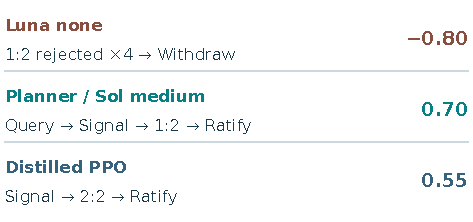
\includegraphics[width=\columnwidth]{figures/discourse_paths.pdf}
\caption{Selected paths under the same Iran-context condition and soft counterpart. Terms $x$:$y$ denote own and reciprocal durations. Values are episode net utility; the learned path uses seed 17.}
\label{fig:discourse}
\end{figure}

Matched Iran-context traces illustrate this distinction (Figure~\ref{fig:discourse}). Luna none repeats a rejected 1:2 offer four times and withdraws, yielding $-0.80$. The planner and Sol medium ask a private question, send a signal, and obtain acceptance of that same offer, yielding 0.70. The question changes the belief from 0.65 to 0; the signal raises the soft counterpart's acceptance utility from $-0.05$ to 0.05. The learned controller instead signals and offers 2:2, yielding 0.55. Wording also matters: in a Syria-context pair, explicit withdrawal terminates the episode, while conditional withdrawal is interpreted as invalid and incurs repeated costs. Appendix~\ref{app:discourse} examines these paths and distinguishes expressed readiness to ratify from ratification itself.

Both types reject the unsignaled 1:2 demand, so repetition provides no new information. A question resolves uncertainty; the subsequent signal makes the demand acceptable. The learned policy instead concedes more. Successful agreement therefore does not establish that it reproduces the planner's information-gathering strategy.
